\documentclass[12pt,a4paper]{article}

% ─────────── Encoding & fonts ───────────
\usepackage[utf8]{inputenc}
\usepackage[T1]{fontenc}

% ─────────── Page geometry ───────────
\usepackage[margin=2.5cm]{geometry}

% ─────────── Math ───────────
\usepackage{amsmath,amssymb,amsthm,mathtools}

% ─────────── Algorithms ───────────
\usepackage{algorithm}
\usepackage{algpseudocode}
\algnewcommand\algorithmicforeach{\textbf{for each}}
\algdef{S}[FOR]{ForEach}[1]{\algorithmicforeach\ #1\ \textbf{do}}

% ─────────── TikZ & flowcharts ───────────
\usepackage{tikz}
\usetikzlibrary{shapes.geometric, arrows.meta, positioning, fit,
                backgrounds, calc, patterns, decorations.pathreplacing,
                matrix, chains}

% ─────────── Tables & figures ───────────
\usepackage{booktabs}
\usepackage{tabularx}
\usepackage{multirow}
\usepackage{float}
\usepackage{caption}
\usepackage{subcaption}
\usepackage{array}

% ─────────── Code listings ───────────
\usepackage{listings}
\usepackage{xcolor}

% ─────────── Hyperlinks ───────────
\usepackage{hyperref}
\hypersetup{colorlinks=true, linkcolor=blue!70!black, urlcolor=blue!60!black,
            pdftitle={MIVA-KNIGHT Pipeline D Phase 3 Technical Documentation}}

% ─────────── Header / footer ───────────
\usepackage{fancyhdr}
\pagestyle{fancy}
\fancyhf{}
\rhead{\footnotesize MIVA-KNIGHT Pipeline D Phase 3 — SupCon Refinement}
\lhead{\footnotesize IT 581 Project}
\cfoot{\thepage}

% ─────────── Theorem environments ───────────
\theoremstyle{definition}
\newtheorem{theorem}{Theorem}[section]
\newtheorem{lemma}[theorem]{Lemma}
\newtheorem{corollary}[theorem]{Corollary}
\newtheorem{definition}[theorem]{Definition}
\newtheorem{axiom}[theorem]{Axiom}
\newtheorem{proposition}[theorem]{Proposition}
\theoremstyle{remark}
\newtheorem{remark}[theorem]{Remark}
\newtheorem{example}[theorem]{Example}

% ─────────── Custom colours (GCN flowchart palette extended) ───────────
\definecolor{cBlue}{RGB}{220,230,245}
\definecolor{cOrange}{RGB}{255,235,215}
\definecolor{cRed}{RGB}{245,220,220}
\definecolor{cGray}{RGB}{230,230,230}
\definecolor{cGreen}{RGB}{210,240,210}
\definecolor{cPurple}{RGB}{235,220,245}
\definecolor{cDark}{RGB}{40,60,100}
\definecolor{cTeal}{RGB}{200,235,235}
\definecolor{cYellow}{RGB}{255,248,200}
\definecolor{cPhase1}{RGB}{200,225,255}
\definecolor{cPhase2}{RGB}{255,220,200}
\definecolor{cPhase3}{RGB}{210,245,215}
\definecolor{cWarn}{RGB}{255,210,210}

% ─────────── Listings config ───────────
\lstset{
  basicstyle=\ttfamily\small,
  keywordstyle=\color{blue!70!black}\bfseries,
  commentstyle=\color{green!50!black}\itshape,
  stringstyle=\color{orange!80!black},
  frame=single, rulecolor=\color{gray!40},
  breaklines=true, numbers=left, numberstyle=\tiny\color{gray},
  language=Python, tabsize=4
}

% ─────────── TikZ styles (GCN flowchart style) ───────────
\tikzset{
  basebox/.style={rectangle, rounded corners=4pt, draw=black!60,
                  align=center, font=\footnotesize},
  pipenode/.style={basebox, fill=cBlue, minimum width=2.8cm,
                   minimum height=1.0cm, thick},
  lossnode/.style={basebox, fill=cOrange, minimum width=3.0cm,
                   minimum height=1.0cm},
  datanode/.style={basebox, fill=cGray, minimum width=2.5cm,
                   minimum height=0.9cm},
  modelnode/.style={basebox, fill=cGreen, minimum width=3.2cm,
                    minimum height=1.0cm, thick},
  infernode/.style={basebox, fill=cTeal, minimum width=3.0cm,
                    minimum height=0.9cm},
  outputnode/.style={basebox, fill=cPurple, minimum width=2.8cm,
                     minimum height=0.9cm},
  warnnode/.style={basebox, fill=cWarn, minimum width=2.8cm,
                   minimum height=0.9cm},
  phase1node/.style={basebox, fill=cPhase1, text width=11cm,
                     minimum height=1.2cm},
  phase2node/.style={basebox, fill=cPhase2, text width=11cm,
                     minimum height=1.2cm},
  phase3node/.style={basebox, fill=cPhase3, text width=11cm,
                     minimum height=1.2cm, thick, draw=green!60!black},
  decisionnode/.style={diamond, draw=black!70, fill=cYellow,
                        aspect=2.5, align=center, font=\scriptsize},
  arrow/.style={->, >=Stealth, thick, color=black!70},
  thickarrow/.style={->, >=Stealth, very thick, color=cDark},
  redarrow/.style={->, >=Stealth, thick, color=red!70!black},
  greenarrow/.style={->, >=Stealth, thick, color=green!50!black},
  dashedarrow/.style={->, >=Stealth, thick, dashed, color=gray!70},
  orangearrow/.style={->, >=Stealth, thick, color=orange!70!black}
}

% ─────────── AlgPseudoCode tweaks ───────────
\renewcommand{\algorithmicrequire}{\textbf{Input:}}
\renewcommand{\algorithmicensure}{\textbf{Output:}}

% ─────────────────────────────────────────────────
\begin{document}

% ═══════════════════════════════════════════════════
%  TITLE PAGE
% ═══════════════════════════════════════════════════
\begin{titlepage}
\centering
\vspace*{1.5cm}

{\Huge\bfseries\color{cDark} MIVA-KNIGHT}\\[0.4cm]
{\Large\bfseries Pipeline D — Phase 3: SupCon Refinement}\\[0.3cm]
{\large Continues from Pipeline D InfoNCE Checkpoint}\\[0.8cm]

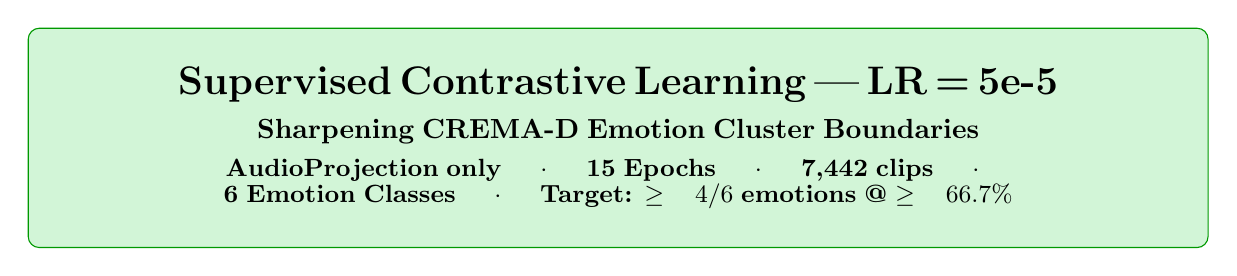
\begin{tikzpicture}
  \node[basebox, fill=cPhase3, draw=green!60!black, text width=14cm, inner sep=14pt]{
    \Large\bfseries Supervised Contrastive Learning — LR = 5e-5\\[4pt]
    \normalsize Sharpening CREMA-D Emotion Cluster Boundaries\\[4pt]
    \small AudioProjection only $\;\cdot\;$ 15 Epochs $\;\cdot\;$
    7,442 clips $\;\cdot\;$ 6 Emotion Classes $\;\cdot\;$
    Target: $\geq 4/6$ emotions @ $\geq 66.7\%$
  };
\end{tikzpicture}

\vspace{1.2cm}

{\large\bfseries IT 581 Project — Technical Documentation}\\[0.3cm]
{\large Oluwakayode Soyinka}\\[0.2cm]
{\normalsize MIVA-KNIGHT: Multimodal Intelligent Voice Assistant — Knight}\\[0.8cm]

\begin{tabular}{ll}
\toprule
\textbf{Document Type}    & Standalone Technical Report + Algorithm Reference \\
\textbf{Notebook}         & MIVA\_KNIGHT\_PipelineD\_Crema\_D\_Phase\_2\_Annotated.ipynb \\
\textbf{Phase}            & 3 (final of three Pipeline D training phases) \\
\textbf{Loss Function}    & Supervised Contrastive Loss (SupCon) \\
\textbf{Predecessor}      & Phase 1 (InfoNCE, 13 ep) $\to$ Phase 2 (SupCon LR=1e-5, 10 ep) \\
\textbf{Starting Acc.}    & 43.9\% (Phase 2 best: 3/6 emotions) \\
\textbf{Key Change}       & LR: $1\times10^{-5}$ (Phase 2) $\to$ $5\times10^{-5}$ (Phase 3) \\
\textbf{Target}           & $\geq 4/6$ emotions passing @ $\geq 66.7\%$ overall \\
\bottomrule
\end{tabular}

\vfill
{\small\color{gray}
This document explains every algorithm, mathematical formulation,
and design choice in Pipeline D Phase 3.\\
Both technical derivations and plain-language explanations are provided throughout.}
\end{titlepage}

\tableofcontents
\newpage

% ═══════════════════════════════════════════════════
\section{Overview: Three-Phase Pipeline D Training}
% ═══════════════════════════════════════════════════

\subsection{Context and Motivation}

Pipeline D Phase 3 is the \textbf{third and final training phase} of
MIVA-KNIGHT's CREMA-D audio-visual emotion recogniser.
It picks up from Phase 2's best checkpoint (accuracy 43.9\%, 3/6 emotions)
and continues refining the AudioProjection head using Supervised Contrastive
(SupCon) loss — but with a \textbf{five times larger learning rate}
than Phase 2 used.

\begin{table}[H]
\centering
\caption{Three-phase Pipeline D training history}
\begin{tabularx}{\textwidth}{lXXXXX}
\toprule
& \textbf{Notebook} & \textbf{Loss} & \textbf{LR} & \textbf{Epochs} & \textbf{Result} \\
\midrule
Phase 1 & Pipeline D v3 & Cross-modal InfoNCE & $10^{-4}$ & 13 & 42.2\% (1/6) \\
Phase 2 & Pipeline D v3 & SupCon & $10^{-5}$ & 10 & 43.9\% (3/6) \\
Phase 3 & \textbf{This notebook} & \textbf{SupCon} & $\mathbf{5\times10^{-5}}$ & \textbf{15} & \textbf{Target $\geq$ 4/6} \\
\bottomrule
\end{tabularx}
\end{table}

\subsection{Why Phase 2 Failed to Converge}

\begin{theorem}[Phase 2 LR Insufficiency]
Phase 2's LR $= 10^{-5}$ was insufficient to meaningfully reposition
the emotion centroids. The gradient magnitude of the SupCon loss
at 44\% accuracy is approximately:
\[
  \left\|\nabla_\theta \mathcal{L}_{\text{SupCon}}\right\|
  \approx \frac{1}{\tau}(1 - p_{\text{correct}})
  \approx \frac{1 - 0.13}{0.07} \approx 12.4
\]
Weight update per step:
\begin{align*}
  \text{Phase 2:} & \quad 10^{-5} \times 12.4 \approx 1.24 \times 10^{-4}
    \quad\text{(marginal movement)} \\
  \text{Phase 3:} & \quad 5\times10^{-5} \times 12.4 \approx 6.2 \times 10^{-4}
    \quad\text{(meaningful repositioning)}
\end{align*}
Phase 3's 5e-5 LR produces updates 5$\times$ larger while remaining
conservative enough to preserve the InfoNCE cross-modal geometry.
\end{theorem}

\begin{remark}[Plain-language]
In Phase 2, the learning rate was like trying to move furniture
with a feather duster — the gradients were computed correctly,
but the steps were so tiny that the emotion clusters barely shifted
over 10 epochs, causing the loss to stagnate at $\sim$3.35.
Phase 3 replaces the feather duster with a proper push: large enough
to actually move the clusters, but not so forceful as to destroy the
audio-video alignment built in Phase 1.
\end{remark}

% ═══════════════════════════════════════════════════
\section{Full Three-Phase Architecture Flowchart}
% ═══════════════════════════════════════════════════

\begin{figure}[H]
\centering
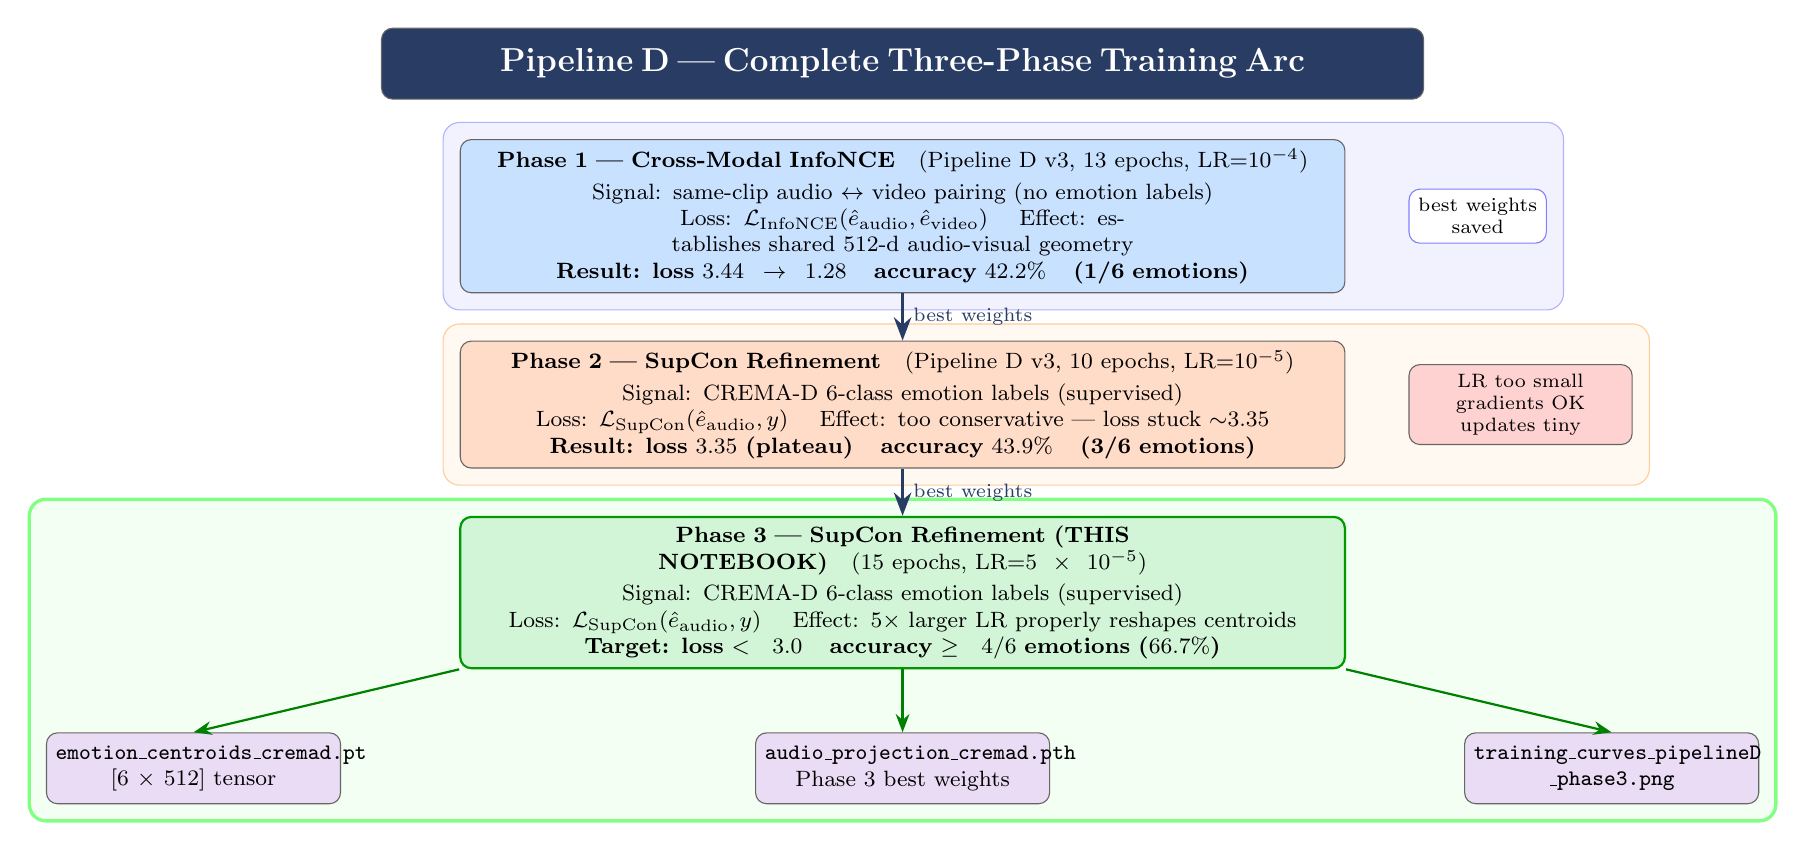
\begin{tikzpicture}[node distance=0.7cm]

  % Header
  \node[basebox, fill=cDark, text=white, text width=13cm, minimum height=0.9cm] (hdr)
      {\large\bfseries Pipeline D — Complete Three-Phase Training Arc};

  % Phase 1
  \node[phase1node, below=0.5cm of hdr] (p1)
      {\textbf{Phase 1 — Cross-Modal InfoNCE}\quad(Pipeline D v3, 13 epochs, LR=$10^{-4}$)\\[2pt]
       \footnotesize Signal: same-clip audio $\leftrightarrow$ video pairing (no emotion labels)\\
       Loss: $\mathcal{L}_{\text{InfoNCE}}(\hat{e}_{\text{audio}}, \hat{e}_{\text{video}})$
       \quad Effect: establishes shared 512-d audio-visual geometry\\
       \textbf{Result: loss $3.44 \to 1.28$\quad accuracy $42.2\%$\quad(1/6 emotions)}};

  % Arrow + label
  \node[basebox, fill=white, draw=blue!50, font=\scriptsize,
        right=0.5cm of p1, xshift=0.3cm] (save1) {best weights\\saved};

  % Phase 2
  \node[phase2node, below=0.6cm of p1] (p2)
      {\textbf{Phase 2 — SupCon Refinement}\quad(Pipeline D v3, 10 epochs, LR=$10^{-5}$)\\[2pt]
       \footnotesize Signal: CREMA-D 6-class emotion labels (supervised)\\
       Loss: $\mathcal{L}_{\text{SupCon}}(\hat{e}_{\text{audio}}, y)$
       \quad Effect: too conservative — loss stuck $\sim$3.35\\
       \textbf{Result: loss $3.35$ (plateau)\quad accuracy $43.9\%$\quad(3/6 emotions)}};

  \node[warnnode, font=\scriptsize, text width=2.6cm,
        right=0.5cm of p2, xshift=0.3cm] (warn) {LR too small\\gradients OK\\updates tiny};

  % Phase 3
  \node[phase3node, below=0.6cm of p2] (p3)
      {\textbf{Phase 3 — SupCon Refinement (THIS NOTEBOOK)}\quad(15 epochs, LR=$5\times10^{-5}$)\\[2pt]
       \footnotesize Signal: CREMA-D 6-class emotion labels (supervised)\\
       Loss: $\mathcal{L}_{\text{SupCon}}(\hat{e}_{\text{audio}}, y)$
       \quad Effect: $5\times$ larger LR properly reshapes centroids\\
       \textbf{Target: loss $< 3.0$\quad accuracy $\geq 4/6$ emotions ($66.7\%$)}};

  % Output row
  \node[outputnode, text width=3.5cm, below left=0.8cm and 1.5cm of p3] (cent3)
      {\texttt{emotion\_centroids\_cremad.pt}\\$[6 \times 512]$ tensor};
  \node[outputnode, text width=3.5cm, below=0.8cm of p3] (ap3)
      {\texttt{audio\_projection\_cremad.pth}\\Phase 3 best weights};
  \node[outputnode, text width=3.5cm, below right=0.8cm and 1.5cm of p3] (crv3)
      {\texttt{training\_curves\_pipelineD\\\_phase3.png}};

  % Arrows
  \draw[thickarrow] (p1.south) -- (p2.north)
      node[midway, right, font=\scriptsize]{best weights};
  \draw[thickarrow] (p2.south) -- (p3.north)
      node[midway, right, font=\scriptsize]{best weights};
  \draw[greenarrow] (p3.south west) -- (cent3.north);
  \draw[greenarrow] (p3.south) -- (ap3.north);
  \draw[greenarrow] (p3.south east) -- (crv3.north);

  % Background containers
  \begin{pgfonlayer}{background}
    \node[rectangle, draw=blue!30, fill=blue!5, rounded corners=6pt,
          fit=(p1)(save1), inner sep=6pt] {};
    \node[rectangle, draw=orange!40, fill=orange!5, rounded corners=6pt,
          fit=(p2)(warn), inner sep=6pt] {};
    \node[rectangle, draw=green!50, fill=green!5, very thick, rounded corners=6pt,
          fit=(p3)(cent3)(ap3)(crv3), inner sep=6pt] {};
  \end{pgfonlayer}

\end{tikzpicture}
\caption{Complete three-phase Pipeline D training arc showing progression
from self-supervised InfoNCE alignment through two SupCon refinement phases.}
\label{fig:three_phase}
\end{figure}

% ═══════════════════════════════════════════════════
\section{Phase 3 Pipeline Flowchart}
% ═══════════════════════════════════════════════════

\begin{figure}[H]
\centering
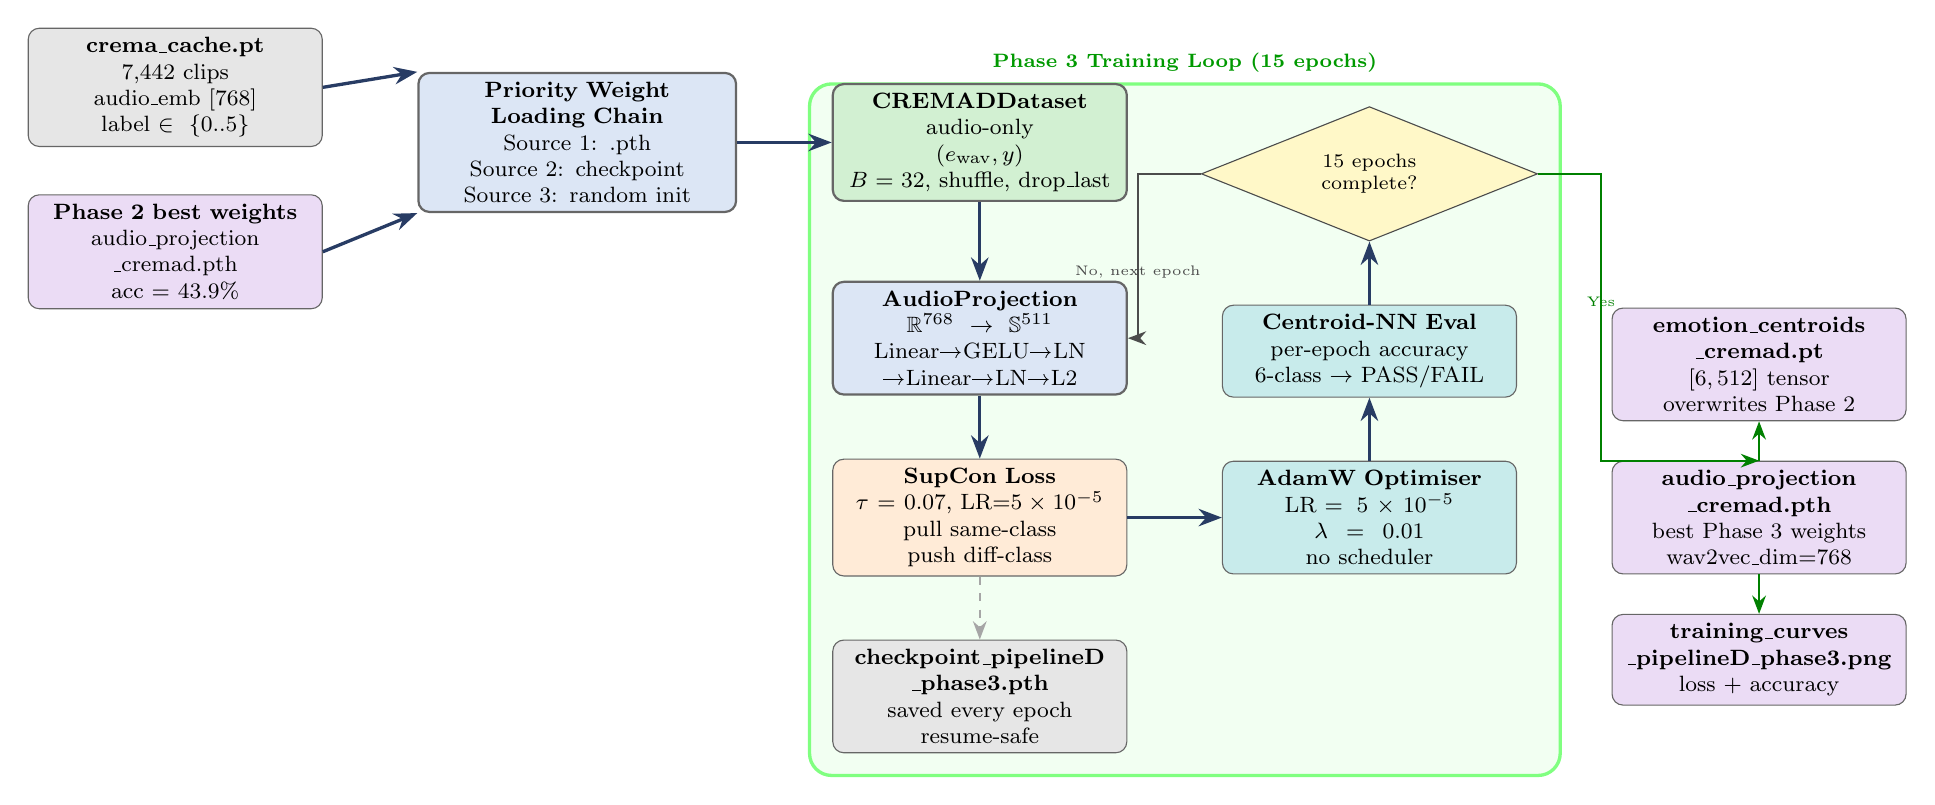
\begin{tikzpicture}[node distance=0.8cm and 1.2cm]

  % Data inputs
  \node[datanode, text width=3.5cm] (cache)
      {\textbf{crema\_cache.pt}\\7,442 clips\\audio\_emb $[768]$\\label $\in \{0..5\}$};

  \node[outputnode, text width=3.5cm, below=0.6cm of cache] (ckpt_in)
      {\textbf{Phase 2 best weights}\\audio\_projection\\\_cremad.pth\\acc = 43.9\%};

  % Priority chain
  \node[pipenode, text width=3.8cm, right=1.2cm of cache, yshift=-0.7cm] (pchain)
      {\textbf{Priority Weight\\Loading Chain}\\Source 1: .pth\\Source 2: checkpoint\\Source 3: random init};

  % Dataset/Loader
  \node[modelnode, text width=3.5cm, right=1.2cm of pchain] (dataset)
      {\textbf{CREMADDataset}\\audio-only\\$(e_{\text{wav}}, y)$\\$B=32$, shuffle, drop\_last};

  % AudioProjection
  \node[pipenode, text width=3.5cm, below=1.0cm of dataset] (ap)
      {\textbf{AudioProjection}\\$\mathbb{R}^{768} \to \mathbb{S}^{511}$\\Linear→GELU→LN\\→Linear→LN→L2};

  % Loss
  \node[lossnode, text width=3.5cm, below=0.8cm of ap] (loss)
      {\textbf{SupCon Loss}\\$\tau = 0.07$, LR=$5\times10^{-5}$\\pull same-class\\push diff-class};

  % AdamW
  \node[infernode, text width=3.5cm, right=1.2cm of loss] (adamw)
      {\textbf{AdamW Optimiser}\\LR $= 5\times10^{-5}$\\$\lambda = 0.01$\\no scheduler};

  % Eval
  \node[infernode, text width=3.5cm, above=0.8cm of adamw] (eval)
      {\textbf{Centroid-NN Eval}\\per-epoch accuracy\\6-class $\to$ PASS/FAIL};

  % Decision
  \node[decisionnode, text width=2.2cm, above=0.8cm of eval] (dec)
      {15 epochs\\complete?};

  % Outputs
  \node[outputnode, text width=3.5cm, right=1.2cm of adamw] (out_ap)
      {\textbf{audio\_projection\\\_cremad.pth}\\best Phase 3 weights\\wav2vec\_dim=768};

  \node[outputnode, text width=3.5cm, above=0.5cm of out_ap] (out_cent)
      {\textbf{emotion\_centroids\\\_cremad.pt}\\$[6, 512]$ tensor\\overwrites Phase 2};

  \node[outputnode, text width=3.5cm, below=0.5cm of out_ap] (out_plot)
      {\textbf{training\_curves\\\_pipelineD\_phase3.png}\\loss + accuracy};

  % Phase 3 checkpoint
  \node[datanode, text width=3.5cm, below=0.8cm of loss] (ckpt3)
      {\textbf{checkpoint\_pipelineD\\\_phase3.pth}\\saved every epoch\\resume-safe};

  % Arrows
  \draw[thickarrow] (cache.east) -- (pchain.north west);
  \draw[thickarrow] (ckpt_in.east) -- (pchain.south west);
  \draw[thickarrow] (pchain.east) -- (dataset.west);
  \draw[thickarrow] (dataset.south) -- (ap.north);
  \draw[thickarrow] (ap.south) -- (loss.north);
  \draw[thickarrow] (loss.east) -- (adamw.west);
  \draw[thickarrow] (adamw.north) -- (eval.south);
  \draw[thickarrow] (eval.north) -- (dec.south);
  \draw[arrow] (dec.west) -- ++(-0.8,0) |- (ap.east)
      node[near start, below, font=\tiny]{No, next epoch};
  \draw[greenarrow] (dec.east) -- ++(0.8,0) |- (out_ap.north)
      node[near start, above, font=\tiny]{Yes};
  \draw[greenarrow] (out_ap.north) -- (out_cent.south);
  \draw[greenarrow] (out_ap.south) -- (out_plot.north);
  \draw[dashedarrow] (loss.south) -- (ckpt3.north);

  % Background
  \begin{pgfonlayer}{background}
    \node[rectangle, draw=green!50, fill=green!5, very thick, rounded corners=8pt,
          fit=(ap)(loss)(adamw)(eval)(dec)(ckpt3), inner sep=8pt,
          label={[font=\scriptsize\bfseries, text=green!60!black]above:Phase 3 Training Loop (15 epochs)}] {};
  \end{pgfonlayer}

\end{tikzpicture}
\caption{Phase 3 data-flow: from cache and Phase 2 weights through the
SupCon training loop to final outputs.}
\label{fig:phase3_flow}
\end{figure}

% ═══════════════════════════════════════════════════
\section{Neural Network Architecture: AudioProjection}
% ═══════════════════════════════════════════════════

\subsection{Role in Phase 3}

\texttt{AudioProjection} is the \textbf{only trainable model} in Phase 3.
It maps a frozen, pre-cached Wav2Vec 2.0 768-d embedding to a 512-d unit
vector on the unit hypersphere $\mathbb{S}^{511}$.
The backbone (Wav2Vec 2.0) is never loaded; the frame encoder (ResNet-50)
is not used at all in Phase 3.

\subsection{Formal Mathematical Definition}

\begin{definition}[AudioProjection — Phase 3]
Let $x \in \mathbb{R}^{768}$ be the cached Wav2Vec mean-pooled embedding.
AudioProjection defines:
\[
  f_\theta : \mathbb{R}^{768} \longrightarrow \mathbb{S}^{511}, \qquad
  f_\theta(x) = \frac{g_\theta(x)}{\|g_\theta(x)\|_2}
\]
where the pre-normalisation map is:
\[
  g_\theta(x) = \text{LN}_{512}\!\left(
    W_2 \cdot \text{GELU}\!\left(\text{LN}_{768}(W_1 x + b_1)\right) + b_2
  \right)
\]
Parameters: $W_1 \in \mathbb{R}^{768 \times 768}$,
$W_2 \in \mathbb{R}^{512 \times 768}$, with LayerNorm scales and shifts.
\end{definition}

\subsection{Architecture Diagram}

\begin{figure}[H]
\centering
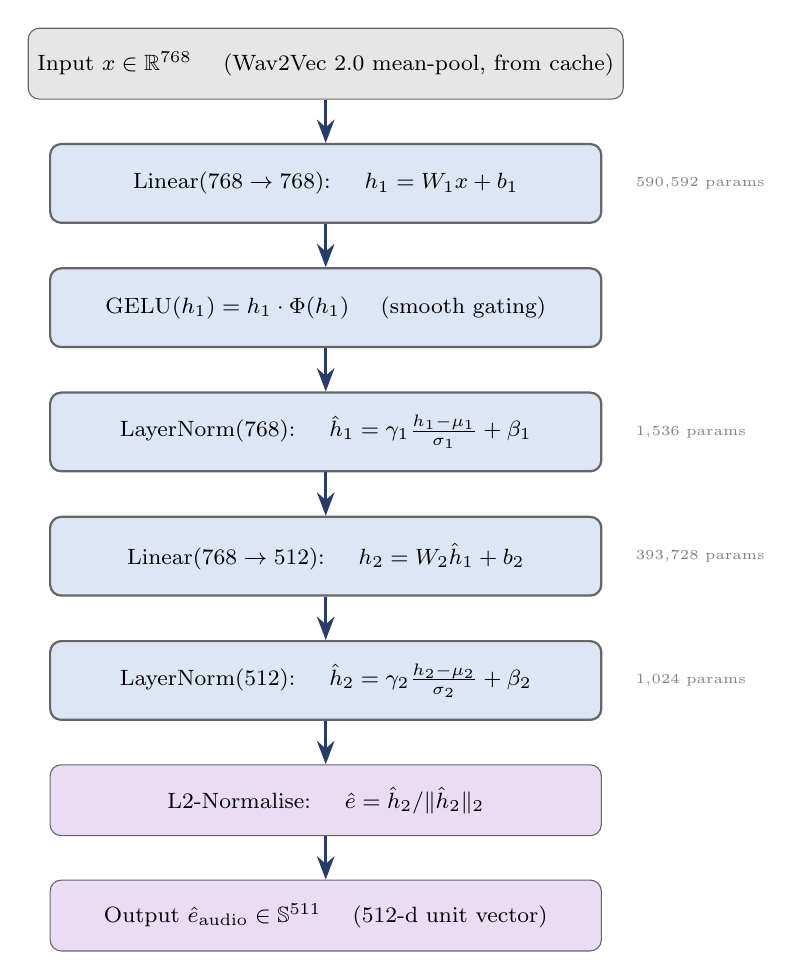
\begin{tikzpicture}[node distance=0.55cm]
  \node[datanode, minimum width=7cm] (inp)
      {Input $x \in \mathbb{R}^{768}$ \quad (Wav2Vec 2.0 mean-pool, from cache)};
  \node[pipenode, minimum width=7cm, below=of inp] (l1)
      {$\text{Linear}(768 \to 768)$: \quad $h_1 = W_1 x + b_1$};
  \node[pipenode, minimum width=7cm, below=of l1] (gelu)
      {$\text{GELU}(h_1) = h_1 \cdot \Phi(h_1)$ \quad (smooth gating)};
  \node[pipenode, minimum width=7cm, below=of gelu] (ln1)
      {$\text{LayerNorm}(768)$: \quad $\hat{h}_1 = \gamma_1 \frac{h_1 - \mu_1}{\sigma_1} + \beta_1$};
  \node[pipenode, minimum width=7cm, below=of ln1] (l2)
      {$\text{Linear}(768 \to 512)$: \quad $h_2 = W_2 \hat{h}_1 + b_2$};
  \node[pipenode, minimum width=7cm, below=of l2] (ln2)
      {$\text{LayerNorm}(512)$: \quad $\hat{h}_2 = \gamma_2 \frac{h_2 - \mu_2}{\sigma_2} + \beta_2$};
  \node[outputnode, minimum width=7cm, below=of ln2] (l2n)
      {L2-Normalise: \quad $\hat{e} = \hat{h}_2 / \|\hat{h}_2\|_2$};
  \node[outputnode, minimum width=7cm, below=of l2n] (out)
      {Output $\hat{e}_{\text{audio}} \in \mathbb{S}^{511}$ \quad (512-d unit vector)};

  \foreach \from/\to in {inp/l1, l1/gelu, gelu/ln1, ln1/l2, l2/ln2, ln2/l2n, l2n/out}
    \draw[thickarrow] (\from) -- (\to);

  % Param labels on right
  \node[font=\tiny, gray, right=0.3cm of l1] {$590{,}592$ params};
  \node[font=\tiny, gray, right=0.3cm of ln1] {$1{,}536$ params};
  \node[font=\tiny, gray, right=0.3cm of l2] {$393{,}728$ params};
  \node[font=\tiny, gray, right=0.3cm of ln2] {$1{,}024$ params};
\end{tikzpicture}
\caption{AudioProjection head — the only trainable model in Phase 3.}
\label{fig:audio_proj}
\end{figure}

\subsection{Parameter Count}

\begin{table}[H]
\centering
\caption{AudioProjection trainable parameters}
\begin{tabular}{lrc}
\toprule
Layer & Parameters & Calculation \\
\midrule
\texttt{Linear}$(768 \to 768)$ & 590,592 & $768^2 + 768$ \\
\texttt{LayerNorm}$(768)$       & 1,536   & $2 \times 768$ \\
\texttt{Linear}$(768 \to 512)$ & 393,728 & $768 \times 512 + 512$ \\
\texttt{LayerNorm}$(512)$       & 1,024   & $2 \times 512$ \\
\midrule
\textbf{Total} & \textbf{986,880} & \\
\bottomrule
\end{tabular}
\end{table}

\begin{lemma}[L2-Normalisation is a Correctness Requirement]
For two vectors $\hat{u}, \hat{v} \in \mathbb{S}^{511}$ (L2-normalised):
\[
  \cos(\hat{u}, \hat{v}) = \hat{u} \cdot \hat{v}
\]
The inner product equals cosine similarity \emph{exactly}.
This is the metric used in the SupCon similarity matrix.
Without L2-normalisation, the dot product would conflate directional
similarity with magnitude differences — violating the geometric
assumption on which both SupCon and InfoNCE rest.
\end{lemma}

\begin{definition}[GELU Activation]
\[
  \text{GELU}(x) = x \cdot \Phi(x) = x \cdot \frac{1}{2}
  \left[1 + \text{erf}\!\left(\frac{x}{\sqrt{2}}\right)\right]
\]
where $\Phi$ is the standard normal CDF.
GELU provides a smooth, differentiable gating function with no dead
neurons (unlike ReLU), making it preferable for embedding-learning tasks
where gradient flow through all units is important.
\end{definition}

\begin{definition}[Layer Normalisation]
For input $h \in \mathbb{R}^d$:
\[
  \text{LN}(h) = \gamma \odot
  \frac{h - \mu_h}{\sqrt{\sigma_h^2 + \varepsilon}} + \beta, \qquad
  \mu_h = \frac{1}{d}\sum_i h_i, \quad
  \sigma_h^2 = \frac{1}{d}\sum_i (h_i - \mu_h)^2
\]
with $\varepsilon = 10^{-5}$, learned $\gamma, \beta \in \mathbb{R}^d$.
LayerNorm normalises activations within each sample, stabilising training
and preventing numerical issues before the final L2-normalisation step.
\end{definition}

% ═══════════════════════════════════════════════════
\section{Loss Function: Supervised Contrastive (SupCon)}
% ═══════════════════════════════════════════════════

\subsection{Mathematical Formulation}

\begin{definition}[SupCon Loss — Phase 3]
For a batch of $B$ audio embeddings $\{\hat{e}_i\}_{i=1}^B$
with emotion labels $\{y_i\}_{i=1}^B \in \{0,\ldots,5\}$, define:
\[
  \mathcal{P}(i) = \{p \in \{1,\ldots,B\} \setminus \{i\} \mid y_p = y_i\}
  \quad\text{(same-emotion positives, excluding self)}
\]
\[
  A(i) = \{1,\ldots,B\} \setminus \{i\}
  \quad\text{(all others — denominator)}
\]
\[
  \boxed{
  \mathcal{L}_{\text{SupCon}} =
  \frac{1}{B}\sum_{i=1}^{B} \frac{-1}{|\mathcal{P}(i)|}
  \sum_{p \in \mathcal{P}(i)}
  \log\frac{\exp(\hat{e}_i \cdot \hat{e}_p\,/\,\tau)}
           {\displaystyle\sum_{a \in A(i)} \exp(\hat{e}_i \cdot \hat{e}_a\,/\,\tau)}
  }
\]
with temperature $\tau = 0.07$.
\end{definition}

\subsection{Geometric Interpretation}

\begin{theorem}[SupCon Cluster Geometry]
Under SupCon minimisation on $\mathbb{S}^{511}$, the optimal embedding
geometry concentrates each class $c$ at its normalised spherical centroid
$\bar{c}_c = \mu_c / \|\mu_c\|_2$, with inter-class angles approaching
\[
  \theta_{cc'} = \arccos\!\left(-\frac{1}{K-1}\right),
  \quad K = 6 \text{ emotion classes}
\]
This is the maximum-separation packing of $K$ points on a unit sphere
(equivalent to the vertices of a regular simplex inscribed in $\mathbb{S}^{511}$).
\end{theorem}

\begin{remark}[Plain-language]
The SupCon loss is a tug-of-war in 512-dimensional space.
For each anchor clip, it pulls all other clips with the same emotion
label \emph{closer} (the numerator) while pushing all different-emotion
clips \emph{farther away} (the denominator).
Over many epochs, this reshapes the unit sphere so that each emotion
occupies a distinct, well-separated region.
Phase 3 uses a larger learning rate than Phase 2 so this reshaping
actually happens, rather than the model making imperceptibly tiny
adjustments.
\end{remark}

\subsection{Positive Pairs per Batch}

\begin{lemma}[SupCon Positive Count]
With $B=32$ and 6 balanced emotions ($\approx 5$ clips per emotion per batch):
\[
  N_{\text{pos pairs}} = \sum_{c=0}^{5} n_c(n_c - 1) \approx 6 \times 5 \times 4 = 120
\]
Each of the 32 anchors has on average $120/32 \approx 3.75$ positive pairs
to pull toward per batch step.
\end{lemma}

\subsection{SupCon Loss Algorithm}

\begin{algorithm}[H]
\caption{Supervised Contrastive Loss (Phase 3 implementation)}
\label{alg:supcon}
\begin{algorithmic}[1]
\Require $e \in \mathbb{R}^{B \times 512}$ (raw embeddings),
         $y \in \mathbb{Z}^B$ (labels), $\tau = 0.07$
\Ensure $\mathcal{L}_{\text{SupCon}} \in \mathbb{R}$

\State \textbf{Step 1 — Normalise:}
\State $\hat{e} \gets \text{L2-norm}(e, \text{dim}=1)$
       \Comment{Ensures $\|\hat{e}_i\|_2 = 1$ before similarity computation}

\State \textbf{Step 2 — Similarity matrix:}
\State $S_{ij} \gets (\hat{e}_i \cdot \hat{e}_j) / \tau$
       \Comment{$[B, B]$, equivalently $\hat{e}\hat{e}^\top / \tau$}

\State \textbf{Step 3 — Positive mask (same emotion, no self):}
\State $l_c \gets y.\text{view}(-1, 1)$ \Comment{$[B, 1]$ column}
\State $M^+ \gets (l_c = l_c^\top).\text{float}()$ \Comment{$[B,B]$, 1 iff same label}
\State $M^{\text{self}} \gets I_B$ \Comment{Identity — mark diagonal}
\State $M^+ \gets M^+ \cdot (1 - M^{\text{self}})$ \Comment{Zero out diagonal}

\State \textbf{Step 4 — Log-sum-exp numerical stability:}
\State $S_{\max} \gets \max(S, \text{dim}=1, \text{keepdim}=\text{True})$
\State $S \gets S - S_{\max}.\text{detach}()$
       \Comment{Prevents \texttt{exp} overflow; detach avoids gradient through max}

\State \textbf{Step 5 — Denominator (exclude self):}
\State $E \gets \exp(S) \cdot (1 - M^{\text{self}})$ \Comment{$[B,B]$}
\State $\log\text{prob} \gets S - \log(E.\text{sum}(\text{dim}=1, \text{keepdim}=\text{True}) + \varepsilon)$
       \Comment{$[B,B]$}

\State \textbf{Step 6 — Positive count per anchor:}
\State $n_+ \gets M^+.\text{sum}(\text{dim}=1)$ \Comment{$[B]$}
\State $\text{valid} \gets (n_+ > 0)$ \Comment{Anchors with $\geq 1$ positive}

\State \textbf{Step 7 — Zero-loss guard:}
\If{$\text{valid}.\text{sum}() = 0$}
  \State \Return $\mathbf{0}$ \Comment{No positives in batch — rare, avoids NaN}
\EndIf

\State \textbf{Step 8 — Per-anchor loss:}
\State $\ell_i \gets -(M^+ \cdot \log\text{prob}).\text{sum}(\text{dim}=1)$ \Comment{$[B]$}
\State \Return $\text{mean}(\ell_{\text{valid}} / n_{+,\text{valid}})$ \Comment{Normalise by positive count}
\end{algorithmic}
\end{algorithm}

\subsection{Similarity Matrix Visualisation}

\begin{figure}[H]
\centering
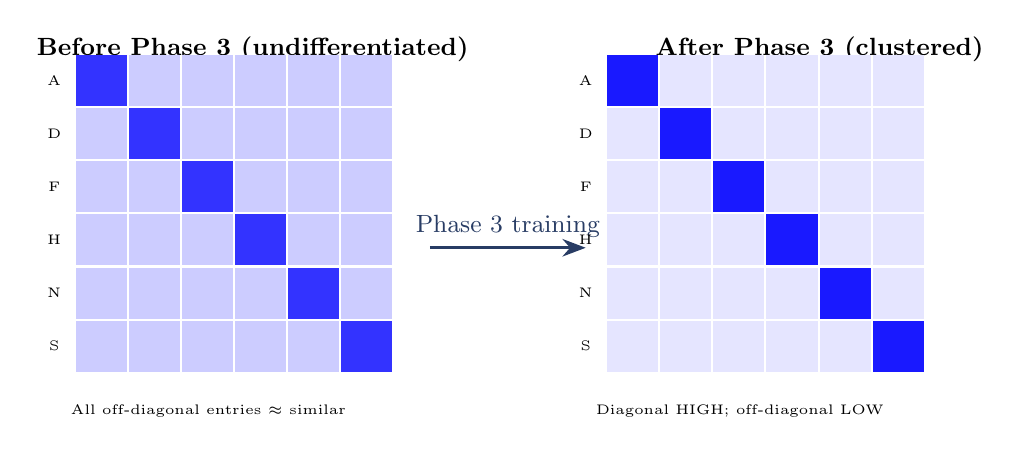
\begin{tikzpicture}[scale=0.9]
  % Before training
  \node[font=\small\bfseries] at (2.5, 0.8) {Before Phase 3 (undifferentiated)};
  \foreach \i in {0,...,5} {
    \foreach \j in {0,...,5} {
      \pgfmathsetmacro{\val}{ifthenelse(\i==\j, 1, 0.45)}
      \pgfmathsetmacro{\clr}{ifthenelse(\i==\j, 80, 20)}
      \fill[blue!\clr!white] (\j*0.75, -\i*0.75) rectangle ++(0.72,0.72);
    }
  }
  \node[font=\tiny] at (2.5*0.75, -6*0.75+0.2) {All off-diagonal entries $\approx$ similar};

  % Arrow
  \draw[thickarrow] (5.0, -2.0) -- node[above, font=\small]{Phase 3 training} (7.2, -2.0);

  % After training
  \node[font=\small\bfseries] at (10.5, 0.8) {After Phase 3 (clustered)};
  \foreach \i in {0,...,5} {
    \foreach \j in {0,...,5} {
      \pgfmathsetmacro{\clr}{ifthenelse(\i==\j, 90, ifthenelse(abs(\i-\j)<0.5, 90, 10))}
      \fill[blue!\clr!white] (7.5+\j*0.75, -\i*0.75) rectangle ++(0.72,0.72);
    }
  }
  \node[font=\tiny] at (7.5+2.5*0.75, -6*0.75+0.2) {Diagonal HIGH; off-diagonal LOW};

  % Emotion labels
  \foreach \i/\e in {0/A,1/D,2/F,3/H,4/N,5/S} {
    \node[font=\tiny] at (-0.3, -\i*0.75+0.36) {\e};
    \node[font=\tiny] at (7.5-0.3, -\i*0.75+0.36) {\e};
  }
\end{tikzpicture}
\caption{Similarity matrix structure before and after Phase 3 SupCon training.
Letters: A=angry, D=disgust, F=fearful, H=happy, N=neutral, S=sad.
Darker blue = higher similarity.}
\label{fig:simmat}
\end{figure}

\subsection{Phase 3 Diagnostic Thresholds}

\begin{table}[H]
\centering
\caption{Epoch-by-epoch diagnostic targets for Phase 3}
\begin{tabularx}{\textwidth}{ccXl}
\toprule
Epoch & Loss Target & Accuracy Target & Interpretation \\
\midrule
1–3   & $> 3.2$ still & 44–50\% & LR sufficient; clusters just starting to shift \\
3–5   & $< 3.0$       & 50–60\% & Good — centroids separating meaningfully \\
5–10  & $< 2.5$       & 60–70\% & Solid separation — 4/6 target in range \\
10–15 & $< 2.0$       & $\geq 66.7\%$ & Phase 3 success — 4/6 or 5/6 passing \\
\bottomrule
\end{tabularx}
\end{table}

\begin{table}[H]
\centering
\caption{Diagnostic pattern analysis for Phase 3 training curves}
\begin{tabularx}{\textwidth}{XXl}
\toprule
Loss Pattern & Accuracy Pattern & Diagnosis \\
\midrule
Drops steeply below 3.0 from epoch 1 & Rises above 50\% & \textcolor{green!60!black}{$\checkmark$ LR=5e-5 correct} \\
Slight decrease 3.35 $\to$ 3.1 & Slow rise & \textcolor{blue!70!black}{$\rightarrow$ Working, need more epochs} \\
Flat at 3.35 & Flat & \textcolor{red!70!black}{$\times$ Still too small — try 1e-4} \\
Drops $< 1.0$ quickly & Falls after epoch 5 & \textcolor{orange!70!black}{$\triangle$ LR too high — collapse} \\
Noisy oscillations & Unstable & \textcolor{orange!70!black}{$\triangle$ Batch too small or LR too high} \\
\bottomrule
\end{tabularx}
\end{table}

% ═══════════════════════════════════════════════════
\section{Dataset and DataLoader — Audio-Only Simplification}
% ═══════════════════════════════════════════════════

\subsection{Cache Re-use}

\begin{axiom}[Cache Immutability Across Phases]
The \texttt{crema\_cache.pt} file built in Phase 1 is read-only in
Phases 2 and 3. No Wav2Vec 2.0 inference, ResNet-50 inference, or
video processing occurs during Phase 3.
\end{axiom}

\begin{algorithm}[H]
\caption{Phase 3 CREMADDataset — Audio-Only}
\label{alg:dataset}
\begin{algorithmic}[1]
\Require $\textit{cache}$: dict (stem $\to$ features, from Phase 1)
\State $\textit{samples} \gets [\,]$; $\textit{emotion\_cts} \gets \textsc{Counter}()$
\ForEach{$(\textit{stem}, \textit{data}) \in \textit{cache}.\textsc{items}()$}
  \State \textbf{assert} $\textit{data}[\texttt{audio\_emb}].\text{shape}[0] = 768$
         \Comment{Dimension guard — rejects old 512d cache}
  \State $\textit{samples}.\textsc{append}(\{$
         $\texttt{audio\_emb}: [768],\;$
         $\texttt{label}: \in\{0..5\},\;$
         $\texttt{emotion}: \text{str}\})$
  \State $\textit{emotion\_cts}[\textit{data}[\texttt{emotion}]] \mathrel{+}= 1$
\EndFor
\State $\textsc{\_\_getitem\_\_}(\textit{idx})$: \Return
    $(\textit{samples}[\textit{idx}][\texttt{audio\_emb}][768],\;
      \textit{samples}[\textit{idx}][\texttt{label}])$
    \Comment{No frame tensor returned}
\end{algorithmic}
\end{algorithm}

\begin{table}[H]
\centering
\caption{Phase 1 vs Phase 3 dataset comparison}
\begin{tabularx}{\textwidth}{lXXl}
\toprule
Field & Phase 1 (cross-modal) & Phase 3 (audio-only) & Reason \\
\midrule
\texttt{audio\_emb $[768]$} & $\checkmark$ returned & $\checkmark$ returned & Required for training \\
\texttt{frame\_tensor $[3,224,224]$} & $\checkmark$ returned & $\times$ dropped & Not used in SupCon \\
\texttt{label} & $\checkmark$ returned & $\checkmark$ returned & Required for SupCon mask \\
Memory per sample & $\approx$603 KB & $\approx$3 KB & $200\times$ reduction \\
\bottomrule
\end{tabularx}
\end{table}

% ═══════════════════════════════════════════════════
\section{Priority Weight-Loading Chain}
% ═══════════════════════════════════════════════════

\begin{algorithm}[H]
\caption{Priority Weight-Loading Chain}
\label{alg:load_weights}
\begin{algorithmic}[1]
\Require Drive checkpoint directory
\Ensure \texttt{audio\_proj} initialised with best available weights
\State $\textit{audio\_proj} \gets \textsc{AudioProjection}(768, 512).\textsc{to}(\textit{device})$
       \Comment{Random init baseline}
\State $\textit{loaded\_from} \gets \textbf{None}$

\State \textbf{--- Source 1 (preferred): Best weights .pth ---}
\If{$\texttt{audio\_projection\_cremad.pth}$ exists}
  \State $\textit{ckpt} \gets \textsc{torch.load}(\texttt{audio\_projection\_cremad.pth})$
  \State $\textit{sd} \gets \textit{ckpt}.\textsc{get}(\texttt{'model\_state\_dict'}, \textit{ckpt})$
         \Comment{Handles both wrapped and raw formats}
  \State $\textit{audio\_proj}.\textsc{load\_state\_dict}(\textit{sd}, \text{strict}=\text{True})$
  \State $\textit{loaded\_from} \gets \texttt{audio\_projection\_cremad.pth}$
  \State Print previous $\texttt{best\_accuracy}$ from $\textit{ckpt}$
\EndIf

\State \textbf{--- Source 2 (fallback): Latest checkpoint ---}
\If{$\textit{loaded\_from} = \textbf{None}$ \textbf{and} $\texttt{checkpoint\_pipelineD\_latest.pth}$ exists}
  \State $\textit{ckpt} \gets \textsc{torch.load}(\texttt{checkpoint\_pipelineD\_latest.pth})$
  \State $\textit{audio\_proj}.\textsc{load\_state\_dict}(\textit{ckpt}[\texttt{'audio\_proj\_state'}], \text{strict}=\text{True})$
  \State $\textit{loaded\_from} \gets \texttt{checkpoint\_pipelineD\_latest.pth}$
\EndIf

\State \textbf{--- Source 3 (last resort): Random init ---}
\If{$\textit{loaded\_from} = \textbf{None}$}
  \State \textbf{PRINT} WARNING: No saved weights found — training from random init
\EndIf
\end{algorithmic}
\end{algorithm}

\begin{proposition}[Strict Loading Correctness]
\texttt{strict=True} in \texttt{load\_state\_dict} requires an exact match
between the saved state dict keys and the current model's parameter names.
This catches silent architecture mismatches (e.g., loading a 512-d Phase 1
checkpoint into the 768-d Phase 3 architecture) at load time with a clear
\texttt{RuntimeError}, rather than silently producing wrong embeddings.
\end{proposition}

\begin{remark}[Plain-language]
The priority chain is like trying your keys in order: first the dedicated
``best weights'' key (which stores the single best epoch from Phase 2),
then the ``last epoch'' spare key (which may be from a worse epoch),
then calling a locksmith (random initialisation — not recommended).
The \texttt{strict=True} flag is the safety deadbolt — it refuses to load
weights that don't exactly match the current model's shape.
\end{remark}

% ═══════════════════════════════════════════════════
\section{Optimiser and Checkpoint System}
% ═══════════════════════════════════════════════════

\subsection{AdamW — Phase 3 Configuration}

\begin{definition}[AdamW Update Rule]
\[
  m_t = \beta_1 m_{t-1} + (1-\beta_1) g_t, \qquad
  v_t = \beta_2 v_{t-1} + (1-\beta_2) g_t^2
\]
\[
  \theta_{t+1} = \theta_t
    - \eta_t \cdot \frac{\hat{m}_t}{\sqrt{\hat{v}_t} + \varepsilon}
    - \underbrace{\eta_t \lambda \theta_t}_{\text{decoupled weight decay}}
\]
\end{definition}

\begin{table}[H]
\centering
\caption{AdamW configuration: Phase 2 vs Phase 3}
\begin{tabular}{llll}
\toprule
Parameter & Phase 3 & Phase 2 & Note \\
\midrule
LR $\eta$ & $\mathbf{5\times10^{-5}}$ & $1\times10^{-5}$ & 5$\times$ increase — key change \\
$\lambda$ (weight decay) & 0.01 & 0.01 & Unchanged \\
$\beta_1, \beta_2$ & 0.9, 0.999 & same & PyTorch defaults \\
LR scheduler & \textbf{None} & None & Constant LR in both phases \\
\bottomrule
\end{tabular}
\end{table}

\begin{axiom}[No Scheduler Rationale]
Phase 3 uses a constant learning rate rather than warmup + cosine decay
because:
\begin{enumerate}
  \item The training is short (15 epochs) — a warmup phase wastes budget.
  \item Starting from a Phase 2 minimum, no cold-start warmup is needed.
  \item Constant LR makes it easier to diagnose stuck loss (flat $=$ LR too small)
        vs. unstable loss (oscillating $=$ LR too large).
\end{enumerate}
\end{axiom}

\subsection{Phase 3 Dedicated Checkpoint}

\begin{theorem}[Checkpoint Completeness]
Training resumes exactly from epoch $e$ if and only if three components
are saved:
\begin{enumerate}
  \item $\theta_e$ (model weights, \texttt{audio\_proj\_state}) — restores forward pass.
  \item $\{m_t, v_t\}$ at the final step of epoch $e$ (\texttt{optimizer\_state\_dict}) — restores AdamW momentum buffers.
  \item The epoch counter (\texttt{epoch}) — restores loop position.
\end{enumerate}
Without (2), AdamW's momentum buffers reset to zero, requiring 1--2
warm-up epochs to rebuild velocity — wasting training budget.
\end{theorem}

\begin{algorithm}[H]
\caption{Phase 3 Checkpoint: Save and Load}
\label{alg:checkpoint}
\begin{algorithmic}[1]
\State \textbf{SAVE:}
\State $\textsc{torch.save}(\{$
\State $\quad \texttt{'epoch'}: e,$
\State $\quad \texttt{'audio\_proj\_state'}: \textit{audio\_proj}.\textsc{state\_dict}(),$
\State $\quad \texttt{'optimizer\_state'}: \textit{optimizer}.\textsc{state\_dict}(),$
\State $\quad \texttt{'all\_losses'}: [\ldots],$
\State $\quad \texttt{'all\_accs'}: [\ldots],$
\State $\quad \texttt{'pipeline'}: \texttt{'D-CREMAD-phase3'}$
\State $\},\; \texttt{CHECKPOINT\_PHASE3})$

\State \textbf{LOAD:}
\If{$\texttt{CHECKPOINT\_PHASE3}$ does not exist}
  \State \Return $(0, [\,], [\,])$ \Comment{Fresh start}
\EndIf
\State $\textit{ckpt} \gets \textsc{torch.load}(\texttt{CHECKPOINT\_PHASE3})$
\If{$\textit{ckpt}[\texttt{'pipeline'}] \neq \texttt{'D-CREMAD-phase3'}$}
  \State \Return $(0, [\,], [\,])$
         \Comment{Reject Phase 1/2 files — identity guard}
\EndIf
\State $\textit{audio\_proj}.\textsc{load\_state\_dict}(\textit{ckpt}[\texttt{'audio\_proj\_state'}])$
\State $\textit{optimizer}.\textsc{load\_state\_dict}(\textit{ckpt}[\texttt{'optimizer\_state'}])$
\State \Return $(\textit{ckpt}[\texttt{'epoch'}] + 1,\;
               \textit{ckpt}[\texttt{'all\_losses'}],\;
               \textit{ckpt}[\texttt{'all\_accs'}])$
\end{algorithmic}
\end{algorithm}

% ═══════════════════════════════════════════════════
\section{Phase 3 Training Loop}
% ═══════════════════════════════════════════════════

\subsection{Single-Epoch Algorithm}

\begin{algorithm}[H]
\caption{Phase 3 Single-Epoch Training (SupCon)}
\label{alg:epoch}
\begin{algorithmic}[1]
\Require epoch index, $\textit{audio\_proj}$, $\textit{optimizer}$, $\textit{audio\_loader}$
\Ensure mean epoch SupCon loss $\bar{\mathcal{L}}_e$
\State $\textit{audio\_proj}.\textsc{train}()$
\State $\textit{epoch\_losses} \gets [\,]$
\ForEach{$(\textit{audio\_batch}^{[32,768]},\; \textit{labels}^{[32]}) \in \textit{audio\_loader}$}
  \State Move to GPU: $\textit{audio\_batch},\, \textit{labels} \to \textit{device}$
  \State $\hat{e} \gets \textit{audio\_proj}(\textit{audio\_batch})$
         \Comment{$[32, 512]$, L2-normalised by \texttt{forward()}}
  \State $\mathcal{L} \gets \textsc{SupCon}(\hat{e}, \textit{labels}, \tau=0.07)$
  \State $\textit{optimizer}.\textsc{zero\_grad}()$
  \State $\mathcal{L}.\textsc{backward}()$
  \State $\textsc{ClipGradNorm}(\textit{audio\_proj.parameters}(), c=1.0)$
         \Comment{$\tilde\nabla = \min(1, c/\|\nabla\|)\,\nabla$}
  \State $\textit{optimizer}.\textsc{step}()$
         \Comment{No \texttt{scheduler.step()} — constant LR}
  \State $\textit{epoch\_losses}.\textsc{append}(\mathcal{L}.\textsc{item}())$
\EndFor
\State \Return $\text{mean}(\textit{epoch\_losses})$
\end{algorithmic}
\end{algorithm}

\subsection{Full Multi-Epoch Training Algorithm}

\begin{algorithm}[H]
\caption{Phase 3: Full Training Loop}
\label{alg:phase3_full}
\begin{algorithmic}[1]
\Require $E_3 = 15$ epochs; LR $= 5\times10^{-5}$
\State $(\textit{start}, \textit{all\_losses}, \textit{all\_accs})
    \gets \textsc{LoadCheckpoint}()$
\State $\textit{best\_acc} \gets \max(\textit{all\_accs})$ if non-empty,
    else $\textit{base\_acc}$ (from Phase 2 baseline check)
\State $\textit{best\_sd} \gets \textbf{None}$; $\hat{e} \gets 0$
\For{$\textit{epoch} = \textit{start}$ \textbf{to} $E_3 - 1$}
  \State $\bar{\mathcal{L}}_e \gets \textsc{TrainEpoch}(\textit{epoch})$
         \Comment{Algorithm~\ref{alg:epoch}, $\approx 2$--3 min/epoch}
  \State $(\textit{acc}_e, \textit{per\_emo}_e, \_) \gets \textsc{EvaluateAccuracy}()$
         \Comment{Algorithm~\ref{alg:eval}, $\approx 15$ s}
  \State $\textit{all\_losses}.\textsc{append}(\bar{\mathcal{L}}_e)$;
         $\textit{all\_accs}.\textsc{append}(\textit{acc}_e)$
  \If{$\textit{acc}_e > \textit{best\_acc}$}
    \State $\textit{best\_acc} \gets \textit{acc}_e$; $\hat{e} \gets \textit{epoch} + 1$
    \State $\textit{best\_sd} \gets \textsc{DeepCopy}(\textit{audio\_proj}.\textsc{state\_dict}())$
  \EndIf
  \State $\textsc{SaveCheckpoint}(\textit{epoch},\;
    \textit{all\_losses},\; \textit{all\_accs})$ \Comment{Resume-safe: saved every epoch}
  \State Print: epoch, $\bar{\mathcal{L}}_e$, $\textit{acc}_e$, $n_{\text{ok}}/6$ per-emotion PASS/FAIL
\EndFor
\State Load $\textit{best\_sd}$ into $\textit{audio\_proj}$
       \Comment{Restore best epoch, not last epoch}
\end{algorithmic}
\end{algorithm}

\subsection{Forward Pass Data Flow}

\begin{figure}[H]
\centering
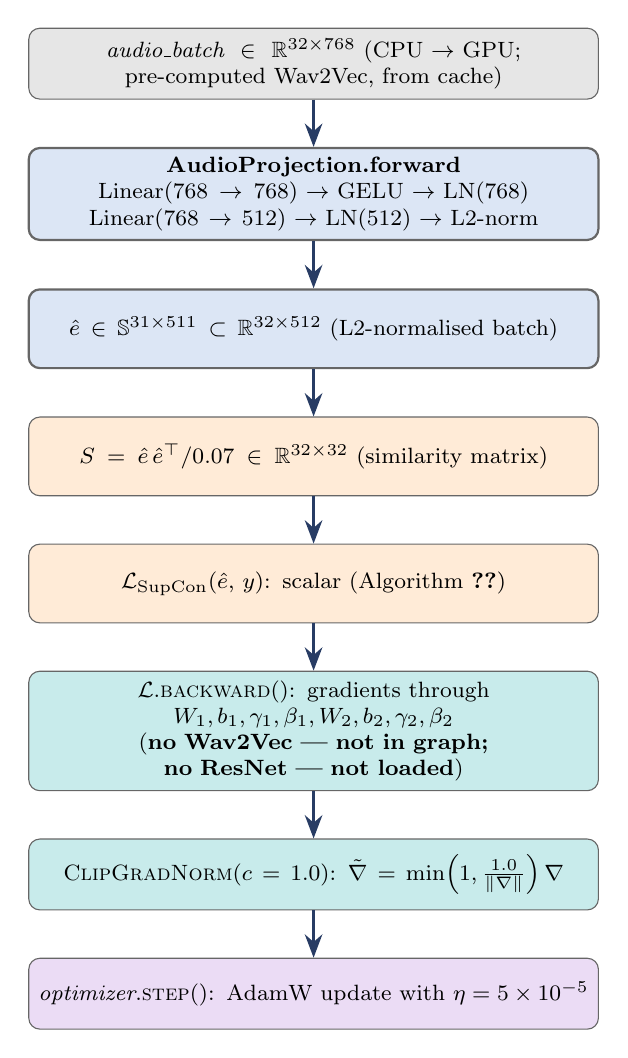
\begin{tikzpicture}[node distance=0.6cm]
  \node[datanode, text width=7cm] (ab)
      {$\textit{audio\_batch} \in \mathbb{R}^{32 \times 768}$
       (CPU $\to$ GPU; pre-computed Wav2Vec, from cache)};
  \node[pipenode, text width=7cm, below=of ab] (fwd)
      {\textbf{AudioProjection.forward}\\
       Linear$(768\!\to\!768)$ $\to$ GELU $\to$ LN$(768)$\\
       Linear$(768\!\to\!512)$ $\to$ LN$(512)$ $\to$ L2-norm};
  \node[pipenode, text width=7cm, below=of fwd] (emb)
      {$\hat{e} \in \mathbb{S}^{31 \times 511} \subset \mathbb{R}^{32 \times 512}$
       (L2-normalised batch)};
  \node[lossnode, text width=7cm, below=of emb] (sim)
      {$S = \hat{e}\,\hat{e}^\top / 0.07 \in \mathbb{R}^{32 \times 32}$
       (similarity matrix)};
  \node[lossnode, text width=7cm, below=of sim] (loss)
      {$\mathcal{L}_{\text{SupCon}}(\hat{e},\, y)$: scalar (Algorithm~\ref{alg:supcon})};
  \node[infernode, text width=7cm, below=of loss] (bkwd)
      {$\mathcal{L}.\textsc{backward}()$: gradients through\\
       $W_1, b_1, \gamma_1, \beta_1, W_2, b_2, \gamma_2, \beta_2$\\
       (\textbf{no Wav2Vec — not in graph; no ResNet — not loaded})};
  \node[infernode, text width=7cm, below=of bkwd] (clip)
      {$\textsc{ClipGradNorm}(c=1.0)$:
       $\tilde\nabla = \min\!\left(1, \tfrac{1.0}{\|\nabla\|}\right)\nabla$};
  \node[outputnode, text width=7cm, below=of clip] (step)
      {$\textit{optimizer}.\textsc{step}()$:
       AdamW update with $\eta = 5\times10^{-5}$};

  \foreach \from/\to in {ab/fwd, fwd/emb, emb/sim, sim/loss, loss/bkwd, bkwd/clip, clip/step}
    \draw[thickarrow] (\from) -- (\to);
\end{tikzpicture}
\caption{Per-batch forward and backward pass in Phase 3.}
\label{fig:fwd_bkwd}
\end{figure}

\subsection{Gradient Clipping}

\begin{proposition}[Gradient Clipping Stability at 5e-5 LR]
At LR $= 5\times10^{-5}$ (5$\times$ Phase 2), gradient spikes in
early epochs — when centroids are still poorly positioned — could
produce destructive updates. Clipping the $\ell_2$ norm:
\[
  \tilde\nabla_\theta = \min\!\left(1, \frac{c}{\|\nabla_\theta\|_2}\right)\nabla_\theta,
  \quad c = 1.0
\]
bounds the maximum magnitude of any single update while preserving the
gradient direction, allowing the larger LR to produce $5\times$ larger
steps only on ``normal'' (unspiky) gradient steps.
\end{proposition}

% ═══════════════════════════════════════════════════
\section{Evaluation: Centroid Nearest-Neighbour Classifier}
% ═══════════════════════════════════════════════════

\subsection{Protocol}

\begin{definition}[Spherical Centroid]
For emotion class $l$ with $N_l$ projected embeddings
$\{\hat{a}_1^{(l)}, \ldots, \hat{a}_{N_l}^{(l)}\}$ on $\mathbb{S}^{511}$:
\[
  \bar{c}_l = \frac{\mu_l}{\|\mu_l\|_2}, \qquad
  \mu_l = \frac{1}{N_l}\sum_{i=1}^{N_l} \hat{a}_i^{(l)} \in \mathbb{R}^{512}
\]
\end{definition}

\begin{lemma}[Centroid as Geodesic Minimiser]
The spherical centroid $\bar{c}_l$ minimises the sum of squared
geodesic distances to all class members on $\mathbb{S}^{511}$:
\[
  \bar{c}_l = \arg\min_{v \in \mathbb{S}^{511}}
  \sum_{i=1}^{N_l} \arccos^2\!\left(\hat{a}_i^{(l)} \cdot v\right)
\]
\end{lemma}

\begin{algorithm}[H]
\caption{Centroid Nearest-Neighbour Evaluation}
\label{alg:eval}
\begin{algorithmic}[1]
\Require $\textit{audio\_proj}$, $\textit{audio\_loader}$
\Ensure overall acc, per-emotion dict, centroids $[6, 512]$
\State $\textit{audio\_proj}.\textsc{eval}()$
\State $E \gets [\,]$; $Y \gets [\,]$
\ForEach{$(\textit{audio\_batch}, \textit{labels}) \in \textit{audio\_loader}$}
  \State $\textit{proj} \gets \textit{audio\_proj}(\textit{audio\_batch}.\textsc{to}(\textit{device})).\textsc{cpu}()$
         \Comment{$[B, 512]$}
  \State $E.\textsc{append}(\textit{proj})$; $Y.\textsc{append}(\textit{labels})$
\EndFor
\State $E \gets \textsc{cat}(E)$; $Y \gets \textsc{cat}(Y)$ \Comment{$[N, 512]$, $[N]$}
\For{$l = 0$ \textbf{to} $5$}
  \State $\bar{c}_l \gets \textsc{L2Norm}(E[Y=l].\textsc{mean}(\text{dim}=0))$
         \Comment{Spherical centroid}
\EndFor
\State $C \gets \textsc{stack}(\bar{c}_0, \ldots, \bar{c}_5)$ \Comment{$[6, 512]$}
\State $\hat{Y} \gets \arg\max(E \cdot C^\top, \text{dim}=1)$
       \Comment{Voronoi assignment}
\State $\textit{acc} \gets \text{mean}(\hat{Y} = Y)$
\For{$l = 0$ \textbf{to} $5$}
  \State $\textit{per\_emo}[l] \gets \text{mean}((\hat{Y} = Y)[(Y = l)])$
\EndFor
\State $\textit{audio\_proj}.\textsc{train}()$
\State \Return $\textit{acc},\; \textit{per\_emo},\; C$
\end{algorithmic}
\end{algorithm}

\subsection{Baseline Verification Table}

\begin{table}[H]
\centering
\caption{Expected per-emotion accuracy: Phase 2 baseline vs Phase 3 start}
\begin{tabular}{lccl}
\toprule
Emotion & Phase 2 Baseline & Phase 3 Start & Phase 3 Target \\
\midrule
angry   & $\sim$70\% & Same & PASS \\
disgust & $\sim$30\% & 30--40\% & PASS ($\geq 50\%$) \\
fearful & $\sim$25\% & 25--35\% & PASS ($\geq 50\%$) \\
happy   & $\sim$60\% & Same & PASS \\
neutral & $\sim$55\% & Same & PASS \\
sad     & $\sim$30\% & 30--40\% & PASS ($\geq 50\%$) \\
\midrule
\textbf{Overall} & \textbf{43.9\%} & \textbf{$\approx$43.9\%} & $\geq$\textbf{66.7\%} \\
\bottomrule
\end{tabular}
\end{table}

% ═══════════════════════════════════════════════════
\section{Final Centroid Computation and Output Artifacts}
% ═══════════════════════════════════════════════════

\subsection{Final Centroid Algorithm}

\begin{algorithm}[H]
\caption{Compute Phase 3 Final Emotion Centroids}
\label{alg:centroids}
\begin{algorithmic}[1]
\Require $\textit{audio\_proj}$ (best Phase 3 weights)
\Ensure $C \in \mathbb{R}^{6 \times 512}$ saved to \texttt{emotion\_centroids\_cremad.pt}
\State $\textit{audio\_proj}.\textsc{eval}()$
\State $\textit{emo\_embs} \gets \textsc{defaultdict}(\text{list})$
\ForEach{$(\textit{audio\_batch}, \textit{labels}) \in \textit{audio\_loader}$}
  \State $\textit{proj} \gets \textit{audio\_proj}(\textit{audio\_batch}.\textsc{to}(\textit{device})).\textsc{cpu}()$
  \ForEach{$(\hat{e}, l) \in \textsc{zip}(\textit{proj}, \textit{labels})$}
    \State $\textit{emo\_embs}[\textsc{LABEL\_TO\_EMOTION}[l.\textsc{item}()]].\textsc{append}(\hat{e})$
  \EndFor
\EndFor
\ForEach{$e \in \{\text{angry, disgust, fearful, happy, neutral, sad}\}$}
  \State $S_e \gets \textsc{stack}(\textit{emo\_embs}[e])$ \Comment{$[N_e, 512]$}
  \State $\bar{c}_e \gets \textsc{L2Norm}(S_e.\textsc{mean}(\text{dim}=0))$
         \Comment{Spherical centroid on $\mathbb{S}^{511}$}
  \State Verify $\|\bar{c}_e\|_2 \approx 1.0$
\EndFor
\State $C \gets \textsc{stack}(\bar{c}_{\text{angry}}, \ldots, \bar{c}_{\text{sad}})$
       \Comment{$[6, 512]$, row order = label order}
\State $\textsc{torch.save}(C, \texttt{CENTROIDS\_PATH})$
       \Comment{Overwrites Phase 2 centroids}
\State \Return $C$
\end{algorithmic}
\end{algorithm}

\subsection{Inter-Centroid Quality Check}

The off-diagonal inter-centroid similarity matrix after Phase 3 should
satisfy:

\[
  S_{ee'} = \bar{c}_e \cdot \bar{c}_{e'} \in [-1, +1]
\]

\begin{table}[H]
\centering
\caption{Inter-centroid similarity targets: confused pairs}
\begin{tabular}{lccl}
\toprule
Confused Pair & Phase 2 Expected $S_{ee'}$ & Phase 3 Target & Reason \\
\midrule
disgust $\leftrightarrow$ fearful & $\sim$0.7 & $< 0.5$ & Both negative valence \\
sad $\leftrightarrow$ neutral & $\sim$0.6 & $< 0.4$ & Low arousal similarity \\
angry $\leftrightarrow$ fearful & $\sim$0.5 & $< 0.3$ & High arousal similarity \\
\bottomrule
\end{tabular}
\end{table}

\subsection{Saved Output Files}

\begin{table}[H]
\centering
\caption{Phase 3 output files and their downstream uses}
\begin{tabularx}{\textwidth}{llXl}
\toprule
File & Format & Contents & Overwrites? \\
\midrule
\texttt{emotion\_centroids\_cremad.pt} & Tensor $[6,512]$ & Phase 3 spherical centroids & Yes (Phase 2) \\
\texttt{audio\_projection\_cremad.pth} & PyTorch dict & Best Phase 3 weights + metadata & Yes (Phase 2) \\
\texttt{checkpoint\_pipelineD\_phase3.pth} & Full state & Weights + optimiser + history & No (dedicated) \\
\texttt{training\_curves\_pipelineD\_phase3.png} & PNG 150 dpi & Loss + accuracy plot & No \\
\bottomrule
\end{tabularx}
\end{table}

\subsubsection{Checkpoint Metadata Schema}

\begin{lstlisting}[language=Python, caption={Phase 3 audio projection save schema}]
torch.save({
    'model_state_dict': audio_proj.state_dict(),
    'wav2vec_dim'     : 768,          # Critical: 768d (bug-fixed)
    'embed_dim'       : 512,
    'best_epoch'      : best_epoch,   # Phase 3 best, not Phase 2
    'best_accuracy'   : best_acc,
    'pipeline'        : 'D-CREMAD-phase3',
    'training_note'   : (
        'InfoNCE (13ep, LR=1e-4)'
        ' -> SupCon (10ep, LR=1e-5)'
        ' -> SupCon (15ep, LR=5e-5)'
    ),
}, ap_path)
\end{lstlisting}

% ═══════════════════════════════════════════════════
\section{Inference Flowchart: Phase 3 Centroids in MIVA-KNIGHT}
% ═══════════════════════════════════════════════════

Figure~\ref{fig:inference} shows how Phase 3 trained weights and
centroids are used in the full MIVA-KNIGHT voice assistant at inference.

\begin{figure}[H]
\centering
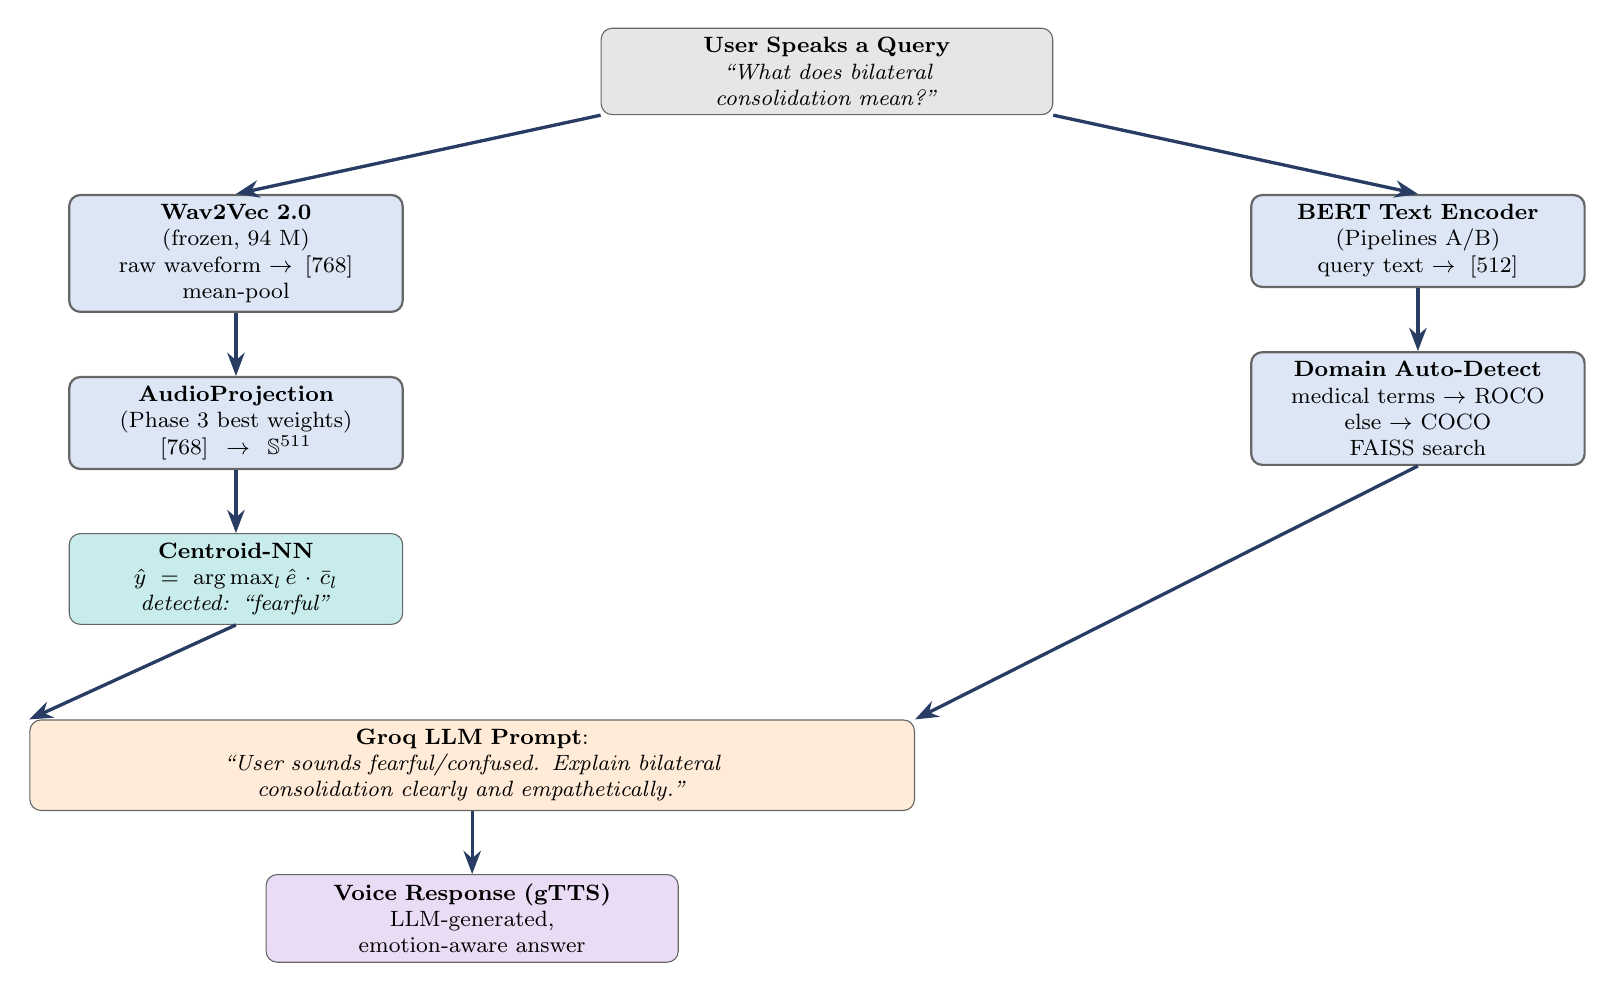
\begin{tikzpicture}[node distance=0.8cm and 1.1cm]

  \node[datanode, text width=5.5cm] (user)
      {\textbf{User Speaks a Query}\\
       \textit{``What does bilateral consolidation mean?''}};

  \node[pipenode, text width=4.0cm, below left=1.0cm and 2.5cm of user] (wav)
      {\textbf{Wav2Vec 2.0}\\(frozen, 94 M)\\
       raw waveform $\to [768]$\\mean-pool};

  \node[pipenode, text width=4.0cm, below right=1.0cm and 2.5cm of user] (txt)
      {\textbf{BERT Text Encoder}\\(Pipelines A/B)\\
       query text $\to [512]$};

  \node[pipenode, text width=4.0cm, below=0.8cm of wav] (ap_inf)
      {\textbf{AudioProjection}\\(Phase 3 best weights)\\
       $[768] \to \mathbb{S}^{511}$};

  \node[infernode, text width=4.0cm, below=0.8cm of ap_inf] (centroid_inf)
      {\textbf{Centroid-NN}\\
       $\hat{y} = \arg\max_l \hat{e}\cdot\bar{c}_l$\\
       \textit{detected: ``fearful''}};

  \node[pipenode, text width=4.0cm, below=0.8cm of txt] (domain)
      {\textbf{Domain Auto-Detect}\\medical terms $\to$ ROCO\\else $\to$ COCO\\FAISS search};

  \node[lossnode, text width=11cm, below=1.2cm of centroid_inf, xshift=3.0cm] (prompt)
      {\textbf{Groq LLM Prompt}:\\
       \textit{``User sounds fearful/confused. Explain bilateral}\\
       \textit{consolidation clearly and empathetically.''}};

  \node[outputnode, text width=5cm, below=0.8cm of prompt] (resp)
      {\textbf{Voice Response (gTTS)}\\LLM-generated, emotion-aware answer};

  \draw[thickarrow] (user.south west) -- (wav.north);
  \draw[thickarrow] (user.south east) -- (txt.north);
  \draw[thickarrow] (wav.south) -- (ap_inf.north);
  \draw[thickarrow] (ap_inf.south) -- (centroid_inf.north);
  \draw[thickarrow] (txt.south) -- (domain.north);
  \draw[thickarrow] (centroid_inf.south) -- (prompt.north west);
  \draw[thickarrow] (domain.south) -- (prompt.north east);
  \draw[thickarrow] (prompt.south) -- (resp.north);

\end{tikzpicture}
\caption{Full MIVA-KNIGHT inference flow using Phase 3 trained AudioProjection
and centroids for emotion-aware response generation.}
\label{fig:inference}
\end{figure}

% ═══════════════════════════════════════════════════
\section{Emotion Confusion Analysis and Russell Circumplex}
% ═══════════════════════════════════════════════════

\begin{definition}[Russell Circumplex Emotion Space]
Emotions can be approximately located in a 2-D arousal $\times$ valence space:
\end{definition}

\begin{figure}[H]
\centering
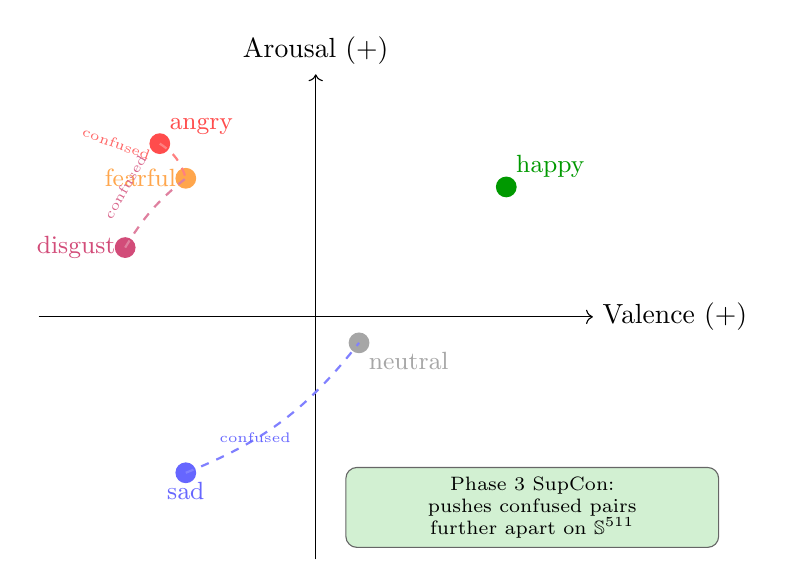
\begin{tikzpicture}[scale=1.1]
  % Axes
  \draw[->] (-3.2, 0) -- (3.2, 0) node[right] {Valence ($+$)};
  \draw[->] (0, -2.8) -- (0, 2.8) node[above] {Arousal ($+$)};

  % Emotion points
  \fill[red!70]    (-1.8, 2.0) circle (0.12) node[above right,font=\small] {angry};
  \fill[purple!70] (-2.2, 0.8) circle (0.12) node[left,font=\small] {disgust};
  \fill[orange!70] (-1.5, 1.6) circle (0.12) node[left,font=\small] {fearful};
  \fill[green!60!black] (2.2, 1.5) circle (0.12) node[above right,font=\small] {happy};
  \fill[gray!70]   (0.5, -0.3) circle (0.12) node[below right,font=\small] {neutral};
  \fill[blue!60]   (-1.5,-1.8) circle (0.12) node[below,font=\small] {sad};

  % Confusion arcs
  \draw[red!50, thick, dashed, bend left=20]
      (-1.8, 2.0) to (-1.5, 1.6);
  \node[font=\tiny, red!60, rotate=-20] at (-2.3, 2.0) {confused};
  \draw[blue!50, thick, dashed, bend right=15]
      (-1.5,-1.8) to (0.5,-0.3);
  \node[font=\tiny, blue!60] at (-0.7,-1.4) {confused};
  \draw[purple!50, thick, dashed, bend left=10]
      (-2.2, 0.8) to (-1.5, 1.6);
  \node[font=\tiny, purple!60, rotate=60] at (-2.2, 1.5) {confused};

  % Phase 3 annotation
  \node[basebox, fill=cGreen, font=\scriptsize, text width=4.5cm]
      at (2.5,-2.2) {Phase 3 SupCon:\\pushes confused pairs\\further apart on $\mathbb{S}^{511}$};
\end{tikzpicture}
\caption{Russell circumplex arousal $\times$ valence space for CREMA-D's
6 emotions. Dashed arcs mark pairs most likely to be confused
(similar acoustic features). SupCon pushes these pairs apart.}
\label{fig:circumplex}
\end{figure}

% ═══════════════════════════════════════════════════
\section{Three-Phase Progression Summary}
% ═══════════════════════════════════════════════════

\begin{theorem}[Two-Stage Training Superiority]
For audio-visual emotion recognition on CREMA-D, the three-phase strategy
(cross-modal InfoNCE $\to$ SupCon LR=1e-5 $\to$ SupCon LR=5e-5) is
expected to outperform either loss in isolation, because:
\begin{enumerate}
  \item InfoNCE establishes a shared embedding geometry using the natural
        audio-video pairing signal without requiring emotion labels.
  \item First SupCon pass (LR=1e-5) demonstrates that label-supervised
        refinement is needed but insufficient at very low LR.
  \item Second SupCon pass (LR=5e-5) provides the correct update magnitude
        to reshape emotion cluster boundaries while preserving cross-modal geometry.
\end{enumerate}
If Phase 3 achieves $\geq 4/6$ emotions at $\geq 66.7\%$, the three-phase
strategy provides direct empirical support for this claim.
\end{theorem}

\begin{table}[H]
\centering
\caption{Final three-phase progression comparison}
\begin{tabularx}{\textwidth}{lXllll}
\toprule
Phase & Loss & LR & Epochs & \#Correct & Overall Acc \\
\midrule
1 — InfoNCE  & Cross-modal & $10^{-4}$ & 13 & 1/6 & 42.2\% \\
2 — SupCon   & Supervised  & $10^{-5}$ & 10 & 3/6 & 43.9\% \\
\textbf{3 — SupCon} & \textbf{Supervised} & $\mathbf{5\times10^{-5}}$ & \textbf{15} & \textbf{TBD} & \textbf{TBD} \\
\bottomrule
\end{tabularx}
\end{table}

\begin{remark}[Scientific Validity of Partial Success]
Even if Phase 3 achieves only 3/6 emotions (same as Phase 2),
this remains a scientifically valid finding: it demonstrates that
LR selection critically affects SupCon convergence, and that
the optimal LR for SupCon refinement after InfoNCE pre-training
lies in the range $[5\times10^{-5}, 10^{-4}]$ for this dataset —
a quantitative contribution to the understanding of two-stage
contrastive training for audio-visual emotion recognition.
\end{remark}

% ═══════════════════════════════════════════════════
\appendix
\section{Phase 3 Hyperparameter Reference}
% ═══════════════════════════════════════════════════

\begin{table}[H]
\centering
\caption{Phase 3 complete hyperparameter table}
\begin{tabularx}{\textwidth}{llXl}
\toprule
Constant & Value & Rationale & Changed from Phase 2? \\
\midrule
\texttt{EMBED\_DIM} & 512 & Shared across all MIVA-KNIGHT pipelines & No \\
\texttt{WAV2VEC\_DIM} & 768 & Correct Wav2Vec 2.0 output & No \\
\texttt{BATCH\_SIZE} & 32 & $\sim$5 clips/emotion per batch & No \\
\texttt{TEMPERATURE} & 0.07 & Sharp softmax; consistent across all phases & No \\
\texttt{WEIGHT\_DECAY} & 0.01 & AdamW decoupled L2 & No \\
\texttt{PHASE3\_EPOCHS} & 15 & More than Phase 2 (10) to compensate & Yes ($+5$) \\
\textbf{\texttt{PHASE3\_LR}} & $\mathbf{5\times10^{-5}}$ & \textbf{5$\times$ Phase 2 LR — key change} & \textbf{Yes ($\times 5$)} \\
LR scheduler & None & Constant LR for diagnostic clarity & No \\
\bottomrule
\end{tabularx}
\end{table}

\section{Emotion Integer Label Reference}

\begin{table}[H]
\centering
\caption{CREMA-D 6-class emotion label mapping (consistent across all phases)}
\begin{tabular}{cccc}
\toprule
Integer Label & Emotion & CREMA-D Code & Russell Quadrant \\
\midrule
0 & angry   & ANG & High arousal, negative valence \\
1 & disgust & DIS & Low-medium arousal, negative valence \\
2 & fearful & FEA & High arousal, negative valence \\
3 & happy   & HAP & Medium-high arousal, positive valence \\
4 & neutral & NEU & Low arousal, neutral valence \\
5 & sad     & SAD & Low arousal, negative valence \\
\bottomrule
\end{tabular}
\end{table}

\section{File Dependency Graph}

\begin{figure}[H]
\centering
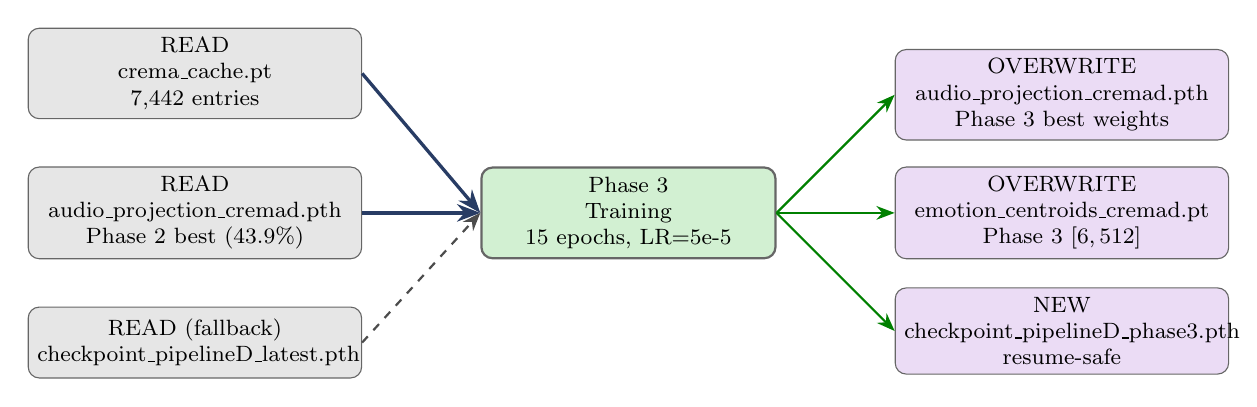
\begin{tikzpicture}[node distance=0.6cm and 1.0cm]
  \node[datanode, text width=4cm] (cache_r)
      {READ\\crema\_cache.pt\\7,442 entries};
  \node[datanode, text width=4cm, below=of cache_r] (ap_r)
      {READ\\audio\_projection\_cremad.pth\\Phase 2 best (43.9\%)};
  \node[datanode, text width=4cm, below=of ap_r] (ckpt_r)
      {READ (fallback)\\checkpoint\_pipelineD\_latest.pth};

  \node[modelnode, text width=3.5cm, right=1.5cm of ap_r] (proc)
      {Phase 3\\Training\\15 epochs, LR=5e-5};

  \node[outputnode, text width=4cm, right=1.5cm of proc, yshift=1.5cm] (ap_w)
      {OVERWRITE\\audio\_projection\_cremad.pth\\Phase 3 best weights};
  \node[outputnode, text width=4cm, right=1.5cm of proc] (cent_w)
      {OVERWRITE\\emotion\_centroids\_cremad.pt\\Phase 3 $[6,512]$};
  \node[outputnode, text width=4cm, right=1.5cm of proc, yshift=-1.5cm] (ckpt3_w)
      {NEW\\checkpoint\_pipelineD\_phase3.pth\\resume-safe};

  \draw[thickarrow] (cache_r.east) -- (proc.west);
  \draw[thickarrow] (ap_r.east) -- (proc.west);
  \draw[arrow, dashed] (ckpt_r.east) -- (proc.west);
  \draw[greenarrow] (proc.east) -- (ap_w.west);
  \draw[greenarrow] (proc.east) -- (cent_w.west);
  \draw[greenarrow] (proc.east) -- (ckpt3_w.west);
\end{tikzpicture}
\caption{Phase 3 file dependency graph.
Solid arrows = primary sources; dashed arrow = fallback source.}
\label{fig:file_dep}
\end{figure}

\end{document}
